\section{Notion avancées}
\label{notion}
L'utilisation de l' ADC peut trouver son utilitée dans la modulation d'une PWM (Pulse Width Modulation) ou  MLI (Modulation de largeur d'impulsions) en français. 
\paragraph{}
Le principe général est qu'en appliquant une succession d'états discrets pendant des durées bien choisies, on peut obtenir en moyenne sur une certaine durée n'importe quelle valeur intermédiaire. un exemple pour une tension d'entrée de 3V vous est présenté à la FIGURE \ref{pwm}.

\begin{figure}[h]
\begin{center}
\begin{framed}
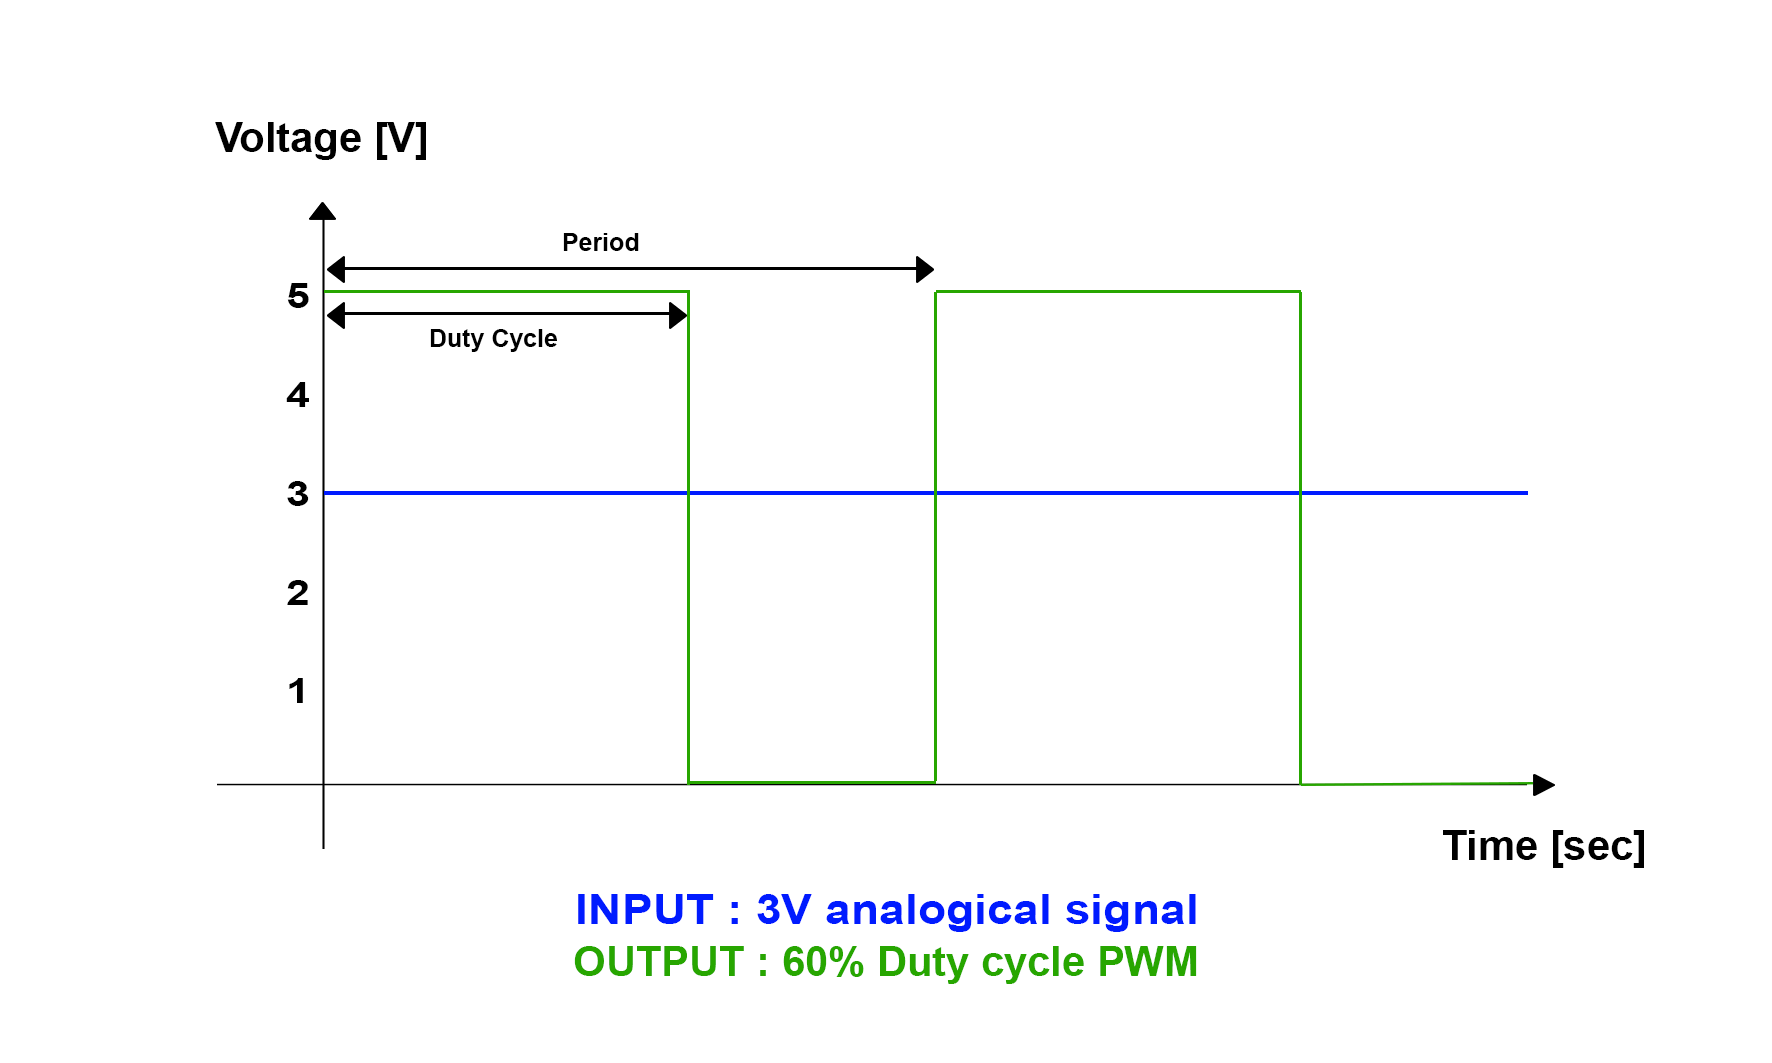
\includegraphics[scale=0.8]{images/pwm.png}
\caption{Transformation d'un signal analogique en signal PWM de tension équivalente}
\label{pwm}
\end{framed}
\end{center}
\end{figure}

\paragraph{}
En se servant de la librairie XC8. Il est très facile d'utiliser le signal numérique de sortie de l'ADC pour créer une PWM. Voici un exemple pour la création d'une PWM :

\paragraph{Création de la PWM} paramétrage de la période\footnote{
le calcul de la durée de la période de la PWM ce fait grâce à la formule $period =[(period ) + 1] x 4 x TOSC x TMR2 prescaler$, cette valeur sera renseignée comme paramètre de la fonction OpenPMMx()} et du mode.
\begin{lstlisting}
OpenPWM1(0xFF);
SetOutputPWM1(SINGLE_OUT, PWM_MODE_1);
\end{lstlisting}

\paragraph{Conversion} On suppose l'ADC correctement paramétré (voir Section \ref{programmation}).
\begin{lstlisting}
ConvertADC();
while(BusyADC());
value = ReadADC();
\end{lstlisting}

\paragraph{on \textit{redirige} notre valeur vers la PWM}.
\begin{lstlisting}
SetDCPWM1(value);
\end{lstlisting}

